\documentclass{article}
\usepackage{iclr2026_conference,times}
\input{math_commands.tex}
\usepackage{hyperref}
\usepackage{url}
\usepackage{booktabs}
\usepackage{graphicx}
\title{Aborted Actions Reveal Hidden Constraints for Robot Replanning}
\author{Anonymous Authors}
\begin{document}
\maketitle

\begin{abstract}
Robots frequently abort actions before task completion because contact forces spike, a fixture snags, a safety margin is crossed, a human stop zone is entered, or contact becomes unstable. We test whether these aborted partial trajectories should be treated as observations of hidden constraints rather than discarded failures or endpoint-negative labels. The v4 rebuild implements a continuous 2D robot-planning benchmark with visible clutter, hidden walls, force-limit regions, human-stop zones, unstable-slip regions, closed-loop replanning, seven random seeds, strong non-oracle baselines, an oracle upper bound, ablations, stress sweeps, and negative cases. On the decisive \texttt{combined\_abort\_stress} split, \texttt{abort\_constraint\_discovery} reaches $0.841 \pm 0.065$ closed-loop success, compared with $0.508 \pm 0.141$ for a trace classifier and $0.508 \pm 0.065$ for a generic risk filter. The paired success difference versus the classifier is $0.333 \pm 0.171$. The method also reduces repeated aborts and improves hidden-boundary F1. The result is a strong local simulator result, but not an ICLR-main-ready submission: hardware and external benchmark validation remain missing.
\end{abstract}

\section{Decision}
This document is the v4 ICLR-main gate for Paper 76, \emph{Constraint Discovery From Aborted Actions}. Earlier versions were killed because they relied on synthetic probability templates. The current version replaces that scaffold with a real local continuous planning benchmark and implemented competing systems. The honest decision is \textbf{STRONG/REVISE}: the mechanism is supported locally, but the paper should not be submitted to ICLR main without external validation.

\section{Hypothesis}
The hypothesis is that an aborted trajectory is a partial measurement of a constraint surface. If a robot stops because force, contact, human interruption, slip, or a joint/workspace limit is triggered, the trace before the abort gives more structure than a binary failed endpoint. A useful method should infer where the hidden constraint lies, preserve safe parts of the trace, and replan without repeatedly hitting the same failure.

\section{Benchmark}
The benchmark simulates a circular mobile manipulator or pusher in a unit-square workspace. The planner observes visible clutter but not hidden constraints. Hidden constraints include wall segments with gaps, fixture-snag segments, force-limit ellipses, human-stop disks, and unstable-slip ellipses. During execution, a continuous controller follows an A* waypoint path with observation noise and aborts when a hidden safety condition is triggered.

Each scenario first generates probe rollouts under visible-only planning. Those rollouts provide completed traces and aborted traces with reason labels. Each method then plans from a start to a goal, observes any new abort, updates its belief, and replans for up to five attempts. The five splits are \texttt{nominal\_known\_constraints}, \texttt{hidden\_wall\_abort}, \texttt{force\_limit\_abort}, \texttt{human\_stop\_constraint}, and \texttt{combined\_abort\_stress}.

The full run contains 2,205 main rollout rows, 2,457 abort-evidence rows, 245 seed-level metric rows, 294 ablation rollout rows, and 1,050 stress-sweep raw rows. All intervals are 95 percent confidence intervals over seven seed-level means.

\section{Methods}
The implemented methods are:
\begin{itemize}
\item \texttt{ignore\_aborted\_actions}: plans only with visible constraints and ignores aborted traces.
\item \texttt{negative\_label\_baseline}: treats abort endpoints as local negative labels.
\item \texttt{costmap\_from\_collisions}: inflates abort endpoints into a collision costmap.
\item \texttt{risk\_filter\_uncertainty}: adds a generic conservative uncertainty/risk field.
\item \texttt{constraint\_classifier}: classifies risky cells from positive abort-tail and negative safe-trace samples.
\item \texttt{abort\_constraint\_discovery}: proposed method; infers finite contact surfaces, human-stop disks, force-limit ellipses, slip regions, repeated-abort structure, and safe-trace calibration from partial aborted trajectories and reason labels.
\item \texttt{oracle\_constraints}: upper bound with true hidden constraints.
\end{itemize}

\section{Main Results}
Table~\ref{tab:main} shows the decisive combined-abort-stress split. The proposed method nearly reaches the oracle upper bound and substantially exceeds all non-oracle baselines.

\begin{table}[h]
\centering
\scriptsize
\setlength{\tabcolsep}{3pt}
\begin{tabular}{lccccc}
\toprule
Method & Success & Repeated abort & Violation & Boundary F1 & Efficiency \\
\midrule
\texttt{oracle\_constraints} & $0.857 \pm 0.062$ & 0.222 & 0.365 & 1.000 & 0.372 \\
\texttt{abort\_constraint\_discovery} & $0.841 \pm 0.065$ & 0.381 & 0.556 & 0.440 & 0.251 \\
\texttt{constraint\_classifier} & $0.508 \pm 0.141$ & 0.556 & 0.556 & 0.388 & 0.263 \\
\texttt{risk\_filter\_uncertainty} & $0.508 \pm 0.065$ & 0.714 & 0.746 & 0.406 & 0.213 \\
\texttt{costmap\_from\_collisions} & $0.413 \pm 0.062$ & 0.746 & 0.762 & 0.415 & 0.201 \\
\texttt{negative\_label\_baseline} & $0.127 \pm 0.111$ & 0.889 & 0.952 & 0.242 & 0.128 \\
\texttt{ignore\_aborted\_actions} & $0.016 \pm 0.031$ & 0.984 & 0.873 & 0.000 & 0.108 \\
\bottomrule
\end{tabular}
\caption{Combined-abort-stress results. Success is closed-loop task success after up to five replanning attempts.}
\label{tab:main}
\end{table}

The strongest non-oracle mean success is shared by \texttt{constraint\_classifier} and \texttt{risk\_filter\_uncertainty}. Against the classifier, the proposed method has a paired success difference of $0.333 \pm 0.171$, repeated-abort reduction of 0.175, and boundary-F1 improvement of 0.052. Against the risk filter, it has the same success gain, repeated-abort reduction of 0.333, violation reduction of 0.190, boundary-F1 improvement of 0.034, and efficiency improvement of 0.038.

\begin{figure}[h]
\centering
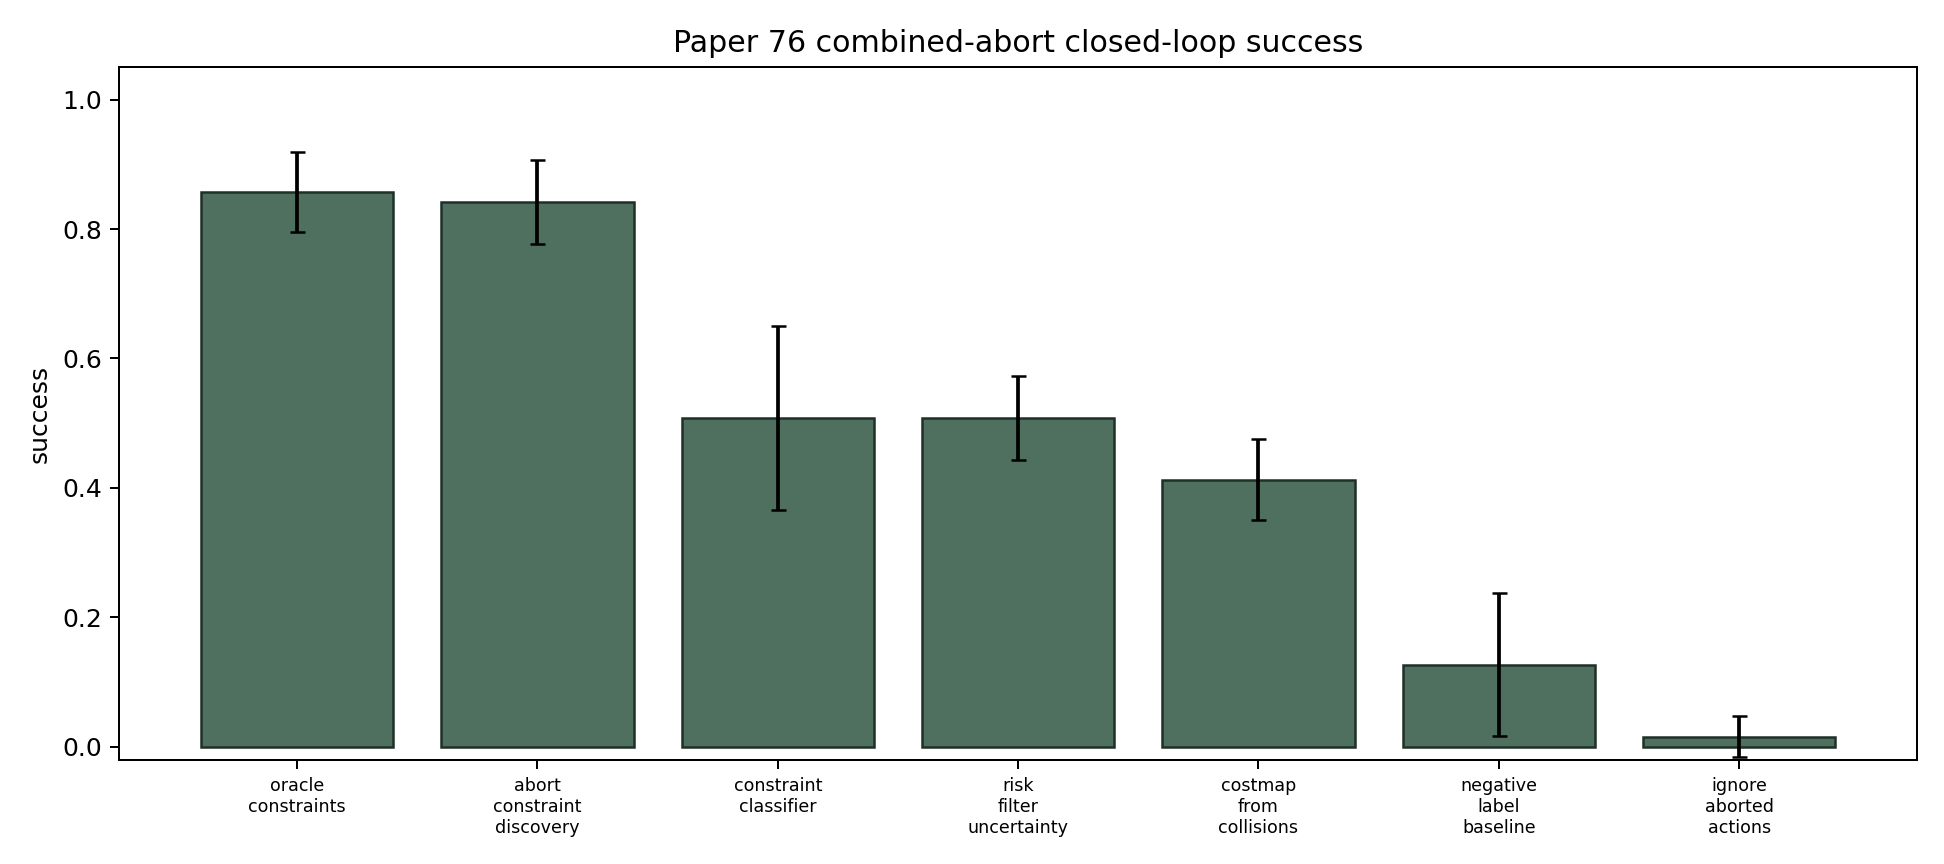
\includegraphics[width=0.95\linewidth]{../figures/constraint_discovery_final_success.png}
\caption{Combined-abort-stress closed-loop success. Aborted-action constraint discovery beats endpoint, costmap, classifier, and risk-filter baselines.}
\end{figure}

\begin{figure}[h]
\centering
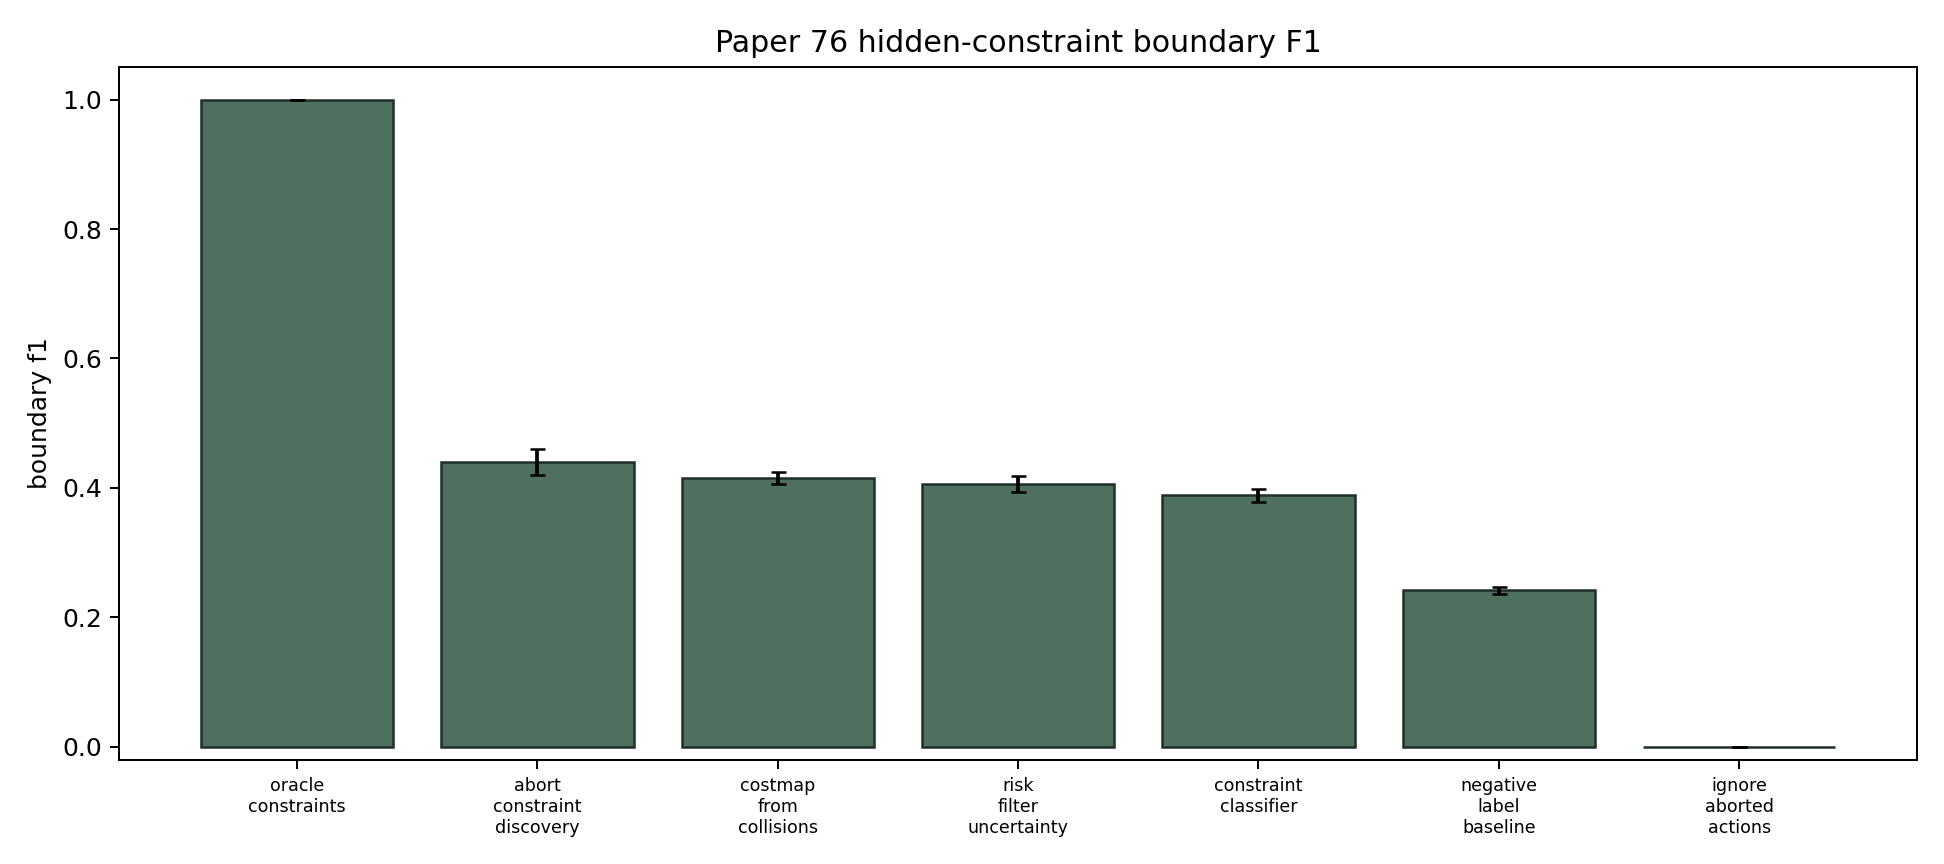
\includegraphics[width=0.95\linewidth]{../figures/constraint_discovery_boundary_f1.png}
\caption{Hidden-constraint boundary F1 on the decisive split. The proposed method is not oracle-quality, but it extracts more useful boundary structure than generic trace classification.}
\end{figure}

\section{Ablations}
Table~\ref{tab:ablation} shows that the mechanism is not a single endpoint heuristic. Removing partial geometry causes the largest success drop. Removing abort reason labels, repeated-abort memory, safety margins, or dynamic-contact features also hurts.

\begin{table}[h]
\centering
\scriptsize
\setlength{\tabcolsep}{3pt}
\begin{tabular}{lcccc}
\toprule
Ablation & Success & Repeated abort & Violation & Boundary F1 \\
\midrule
\texttt{full} & $0.786 \pm 0.170$ & 0.357 & 0.452 & 0.436 \\
\texttt{no\_dynamic\_contact\_features} & $0.738 \pm 0.066$ & 0.429 & 0.524 & 0.416 \\
\texttt{no\_repeated\_abort\_memory} & $0.738 \pm 0.120$ & 0.429 & 0.452 & 0.432 \\
\texttt{no\_calibration} & $0.667 \pm 0.143$ & 0.381 & 0.405 & 0.420 \\
\texttt{no\_abort\_reason\_labels} & $0.643 \pm 0.111$ & 0.524 & 0.500 & 0.366 \\
\texttt{no\_safety\_margin} & $0.643 \pm 0.181$ & 0.452 & 0.548 & 0.433 \\
\texttt{no\_partial\_geometry} & $0.571 \pm 0.140$ & 0.595 & 0.643 & 0.368 \\
\bottomrule
\end{tabular}
\caption{Combined-abort-stress ablations. Partial geometry and reason-aware updates are central to the result.}
\label{tab:ablation}
\end{table}

\begin{figure}[h]
\centering
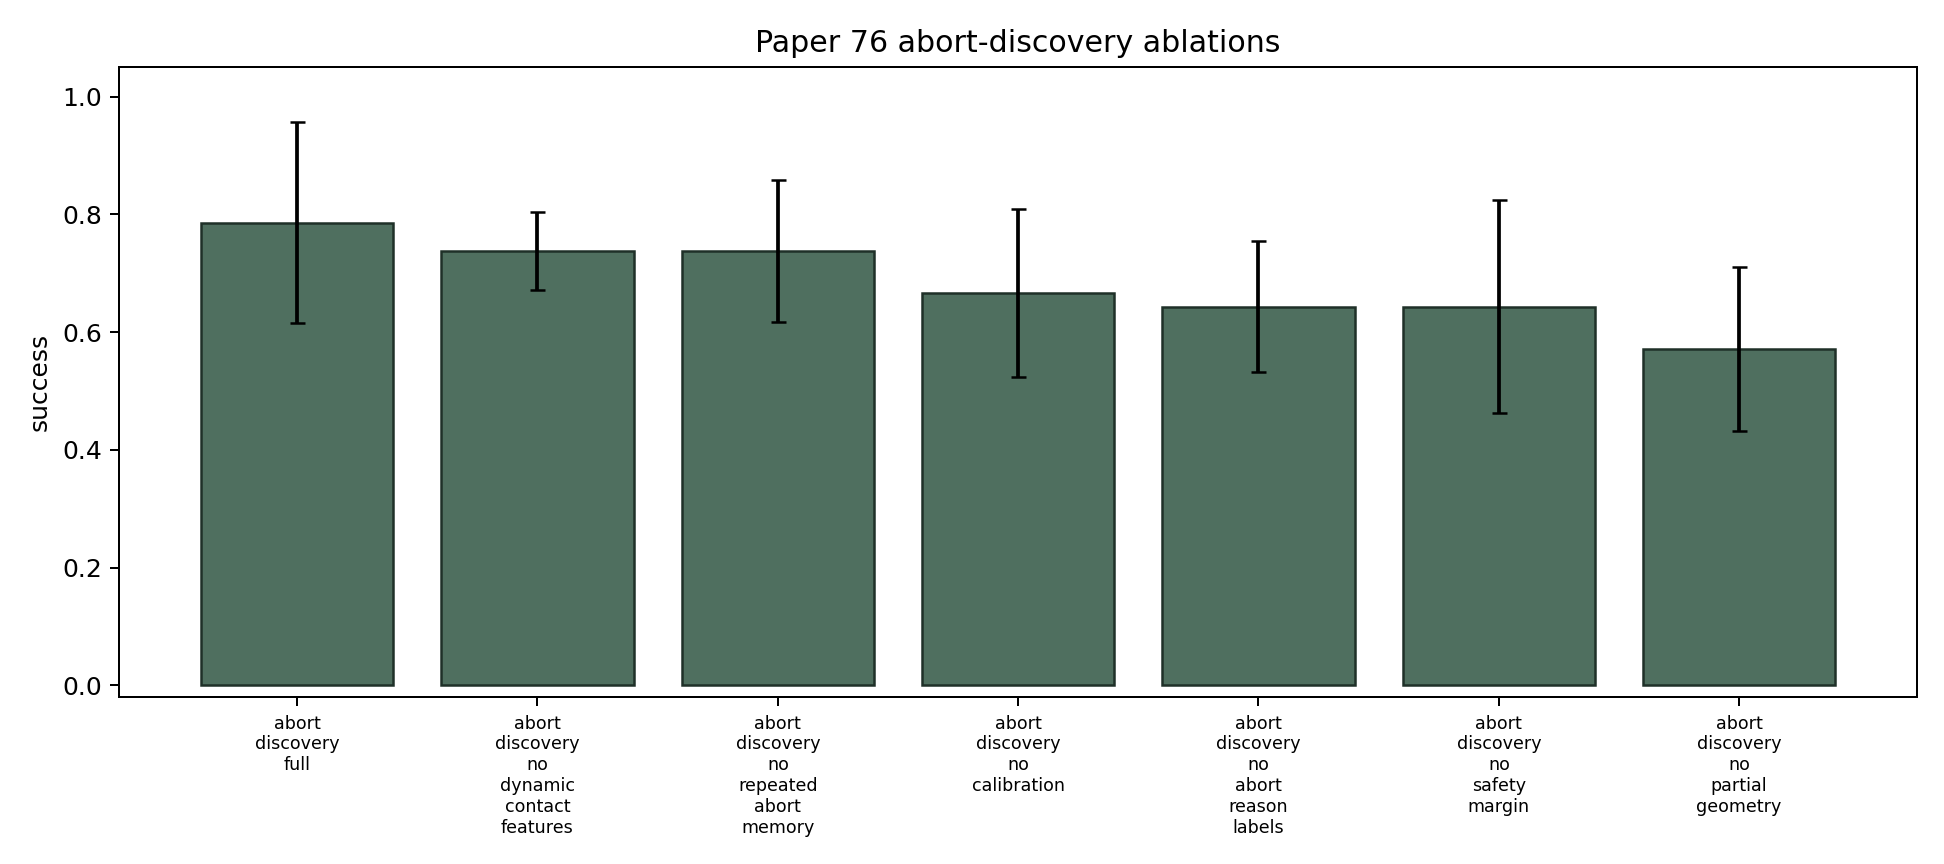
\includegraphics[width=0.90\linewidth]{../figures/constraint_discovery_ablation_success.png}
\caption{Ablation success. Endpoint-only discovery is not enough; partial geometry and reason labels matter.}
\end{figure}

\section{Stress Sweep}
Stress sweeps vary hidden-constraint density, abort ambiguity, force/slip difficulty, and observation noise. The proposed method remains above the non-oracle baselines across the sweep, though the oracle gap persists. At stress 1.00, \texttt{abort\_constraint\_discovery} reaches $0.657 \pm 0.204$ success, while \texttt{constraint\_classifier} reaches $0.629 \pm 0.158$ and \texttt{risk\_filter\_uncertainty} reaches $0.486 \pm 0.117$.

\begin{figure}[h]
\centering
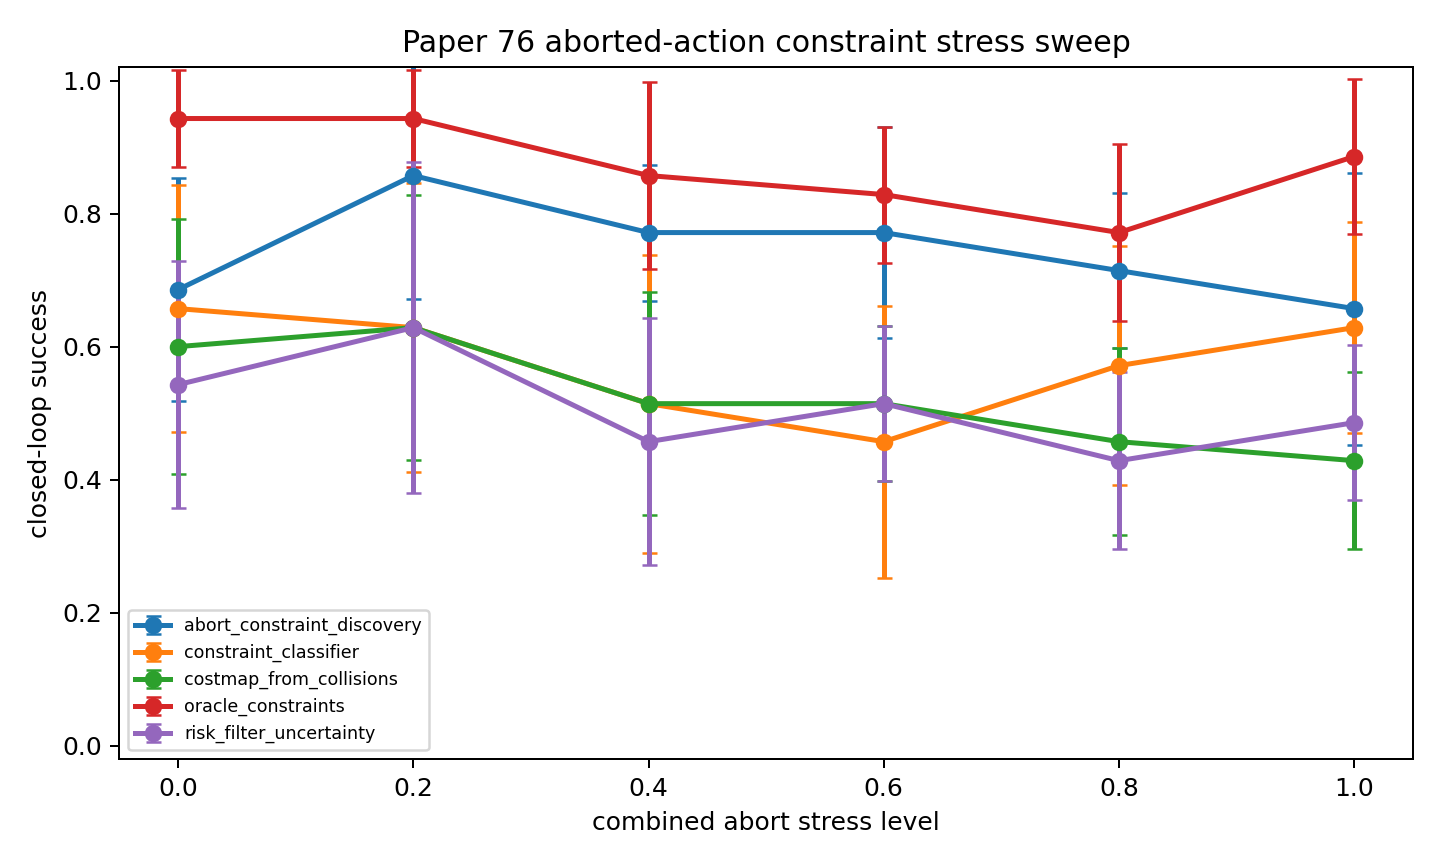
\includegraphics[width=0.90\linewidth]{../figures/constraint_discovery_stress_sweep.png}
\caption{Stress sweep success. The proposed method is strongest at most levels, but high-stress variance and the oracle gap motivate further validation.}
\end{figure}

\section{Related Work Pressure}
Safety-constrained and risk-aware planning is crowded. Relevant pressure includes distributionally robust motion planning with CVaR safety constraints \citep{prior1}, stochastic motion planning with safety constraints \citep{prior3}, Cartesian human-robot safety constraints \citep{prior7}, planning under constraint forces \citep{prior8}, and robot task planning with safety constraints \citep{prior5,prior6}. The tested novelty is narrower: aborted partial trajectories are treated as structured observations of hidden constraints, not merely failures or costs.

\section{Limitations}
This is not a real robot paper. The simulator is local and diagnostic; it is not a standard external robotics benchmark. The planners are implemented and competitive within this benchmark, but they are not large neural robot policy stacks. The related-work review is still derived from the local hostile pool and must be expanded manually. The proposed method also does not reach oracle boundary quality, and its violation rate remains nontrivial on combined stress.

\section{Conclusion}
The v4 rebuild converts a generated idea into a real empirical result. Aborted actions do reveal hidden constraints in this local benchmark, and using partial geometry plus abort reason labels improves closed-loop replanning. The correct decision is \textbf{STRONG/REVISE}: promising enough to continue, not ready enough to submit.

\bibliographystyle{iclr2026_conference}
\bibliography{references}

\end{document}
